\section{Logical View}

The logical view provides a conceptual model of the software's architecture and its components. 
This includes how the software is organized and how its different parts work together.
This will be the largest section of the document.

\begin{figure}[h]
    \centering
    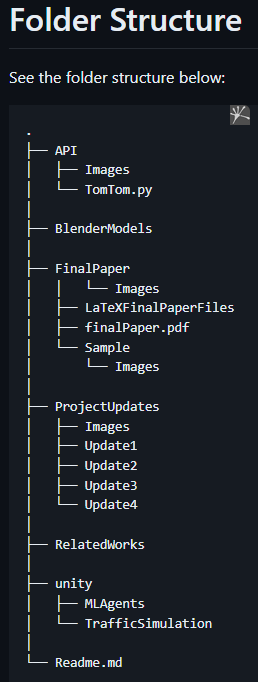
\includegraphics[height=13cm]{Images/FolderStructure.png}
       \caption{Folder Structure of the project.}
           \label{Fig:ProjHier}
\end{figure}

\subsection{High-Level Design (Architecture)}

\begin{figure}[htb]
    \centering
    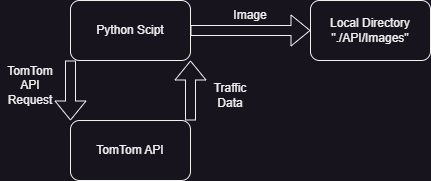
\includegraphics[width=10cm]{Images/TomTomLogFlow.png}
       \caption{Hierarchy of the script.}
           \label{Fig:TomTomHier}
\end{figure}

Another diagram be a layered image for each section of the project from unity to connecting to the python script, pathfinding, etc. each layer should be explained as well.

\subsubsection{TomTom.py}

Below is a class diagram of the TomTom API.

\begin{figure}[htb]
    \centering
    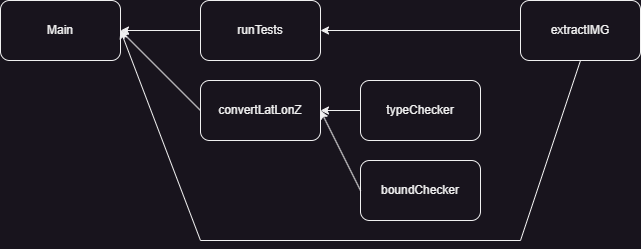
\includegraphics[width=10cm]{Images/TomTomHier.png}
       \caption{Hierarchy of the script.}
           \label{Fig:TomTomHier}
\end{figure}

\newpage

\subsection{Detailed Class Design}

should show a list of all functions and classes used to create the project

all classes/functions should have:
-Inputs
-Purpose
-Output

\subsubsection{TomTom.py}

\begin{itemize}

    \item extractIMG

    \begin{itemize}
        
        \item \textbf{Inputs}: (\textit{String}) HTML link, (\textit{Boolean}) Save the image if true

        \item \textbf{Purpose}: given the HTML link, connects to the TomTom API to obtain the desired image. If instructed, will also save the image in the local folder: './API/Images'

        \item \textbf{Output}: N/A

    \end{itemize}
    
    \item boundChecker

    \begin{itemize}
        
        \item \textbf{Inputs}: (\textit{Float}) Latitude, (\textit{Float}) Longitude, (\textit{Int}) Zoom level, (\textit{String}) Style of image, (\textit{Boolean}) Verbose option. If true prints to console about checking bounds for given inputs

        \item \textbf{Purpose}: Ensures proper bounds on the given inputs

        \item \textbf{Output}: (\textit{Boolean}) True means that the inputs are properly within the bounds

    \end{itemize}
    
    \item typeChecker

    \begin{itemize}
        
        \item \textbf{Inputs}: (\textit{Float}) Latitude, (\textit{Float}) Longitude, (\textit{Int}) Zoom level, (\textit{String}) Style of image, (\textit{Boolean}) Verbose option. If true prints to console about checking types for given inputs

        \item \textbf{Purpose}: Checks the types for all parameters given

        \item \textbf{Output}: (\textit{Boolean}) True means that the inputs are of the proper type

    \end{itemize}
    
    \item convertLatLonZ

    \begin{itemize}
        
        \item \textbf{Inputs}: (\textit{Float}) Latitude, (\textit{Float}) Longitude, (\textit{Int}) Zoom level, (\textit{String}) Style of image, (\textit{Boolean}) Verbose option. If true prints to console about converting parameters to proper format

        \item \textbf{Purpose}: Determines the coordinates to use according to the zoom level. This information is needed when accessing the API to obtain the correct location information \cite{ConversionTomTom}. 

        \item \textbf{Output}: (\textit{Tuple}) Tuple of 3 elements: X, Y, Zoom level

    \end{itemize}

    \item heightCalc

    \begin{itemize}
        
        \item \textbf{Inputs}: (\textit{Int}) Red value of pixel, (\textit{Int}) Green value of pixel, (\textit{Int}) Blue value of pixel

        \item \textbf{Purpose}: Determines the height of a given pixel given the RGB values of the image. This formula is from TomTom \cite{HeightCalcTomTom}. Unused in the final product

        \item \textbf{Output}: (\textit{Float}) Height of the region described by the pixel as feet above sea level

    \end{itemize}

    \item runTests

    \begin{itemize}
        
        \item \textbf{Inputs}: (\textit{Boolean}) Save the images if true, (\textit{Boolean}) Verbose option. Print to the console about each step

        \item \textbf{Purpose}: Will run a series of tests with default locations to show the different options available for this script

        \item \textbf{Output}: N/A

    \end{itemize}

    \item main

    \begin{itemize}
        
        \item \textbf{Inputs}: (\textit{String}) Latitude, (\textit{String}) Longitude, (\textit{String}) Zoom Level, (\textit{String}) Style of Image to produce, (\textit{Boolean}) Save image created if true, (\textit{String}) Run demo options to showcase all options from this script if true, (\textit{String}) Verbose. If true, describes the steps occurring in the program as they occur

        \item \textbf{Purpose}: Parses the given arguments, runs through each of the above described functions to achieve the goal of obtaining the image with the given arguments

        \item \textbf{Output}: N/A

    \end{itemize}

\end{itemize}